%!TeX encoding=utf8
\documentclass[ngerman]{scrartcl} 

\newcommand{\authA}{Daniel Scheiermann}
\newcommand{\matA}{3227680}
\newcommand{\authB}{Felix Springer}
\newcommand{\matB}{10002537}
\newcommand{\grpnr}{SLOT}
\newcommand{\Versuchsnummer}{IQ18}
\newcommand{\Versuchsname}{Scanning Laser Optical Tomography}


%%%%%%%%%%%%%%%%%%Capitalized Color - start%%%%%%%%%%%%%%%%%%%%%%%%
\usepackage{xparse}
\usepackage{xcolor}


\ExplSyntaxOn
\NewDocumentCommand{\colorcap}{ O{blue} m }
 {
  \sheljohn_colorcap:nn { #1 } { #2 }
 }

\tl_new:N \l__sheljohn_colorcap_input_tl
\cs_new_protected:Npn \sheljohn_colorcap:nn #1 #2
 {
  % store the string in a variable for usage with \regex_replace_all:nnN
  \tl_set:Nn \l__sheljohn_colorcap_input_tl { #2 }
  \regex_replace_all:nnN
   { ([A-Z]+) } % search a capital letter (or more)
   { \c{textcolor}\cB\{#1\cE\}\cB\{\1\cE\} } % replace the match with \textcolor{#1}{<match>}
   \l__sheljohn_colorcap_input_tl
  \tl_use:N \l__sheljohn_colorcap_input_tl
 }
\ExplSyntaxOff
%%%%%%%%%%%%%%%%%%Capitalized Color - end%%%%%%%%%%%%%%%%%%%%%%%%
%---configure pagelayout
\KOMAoptions{ % read documentation for KOMAScript providing the documentclass scrartcl
DIV=11,
BCOR=0mm,
paper=a4,
fontsize=12pt,
parskip=half,
twoside=false,
titlepage=true
}

%\usepackage[ %Set linespacing
%singlespacing %onehalfspacing,doublespacing
%]{setspace} 

\usepackage[headsepline,footsepline,automark,pagestyleset=KOMA-Script,markcase=ignoreuppercase]{scrlayer-scrpage} %Configure headline and footer

\clearscrheadings
\setlength{\headheight}{3.5\baselineskip}

\ihead[]{\authB~(\matB)\\\authA~(\matA)}
\ohead{
\includegraphics[height=13pt]{IMAGE/luh_logo.png} \\ \Versuchsnummer $ $ \grpnr}

\cfoot{\vspace{-0.75cm}\pagemark}
\pagestyle{scrheadings}

%better positioning of floatings
\renewcommand{\floatpagefraction}{.75} % standard: .5
\renewcommand{\textfraction}{.1} % standard: .2
\renewcommand{\topfraction}{.8} % standard: .7
\renewcommand{\bottomfraction}{.5} % standard: .3
\setcounter{topnumber}{3} % standard: 2
\setcounter{bottomnumber}{2} % standard: 1
\setcounter{totalnumber}{5} % standard: 3

%---Language and umlauts
\usepackage[utf8]{inputenc} %Set UTF-8 encoding, enables ä,ö,ü etc.
\usepackage[ngerman]{babel} %Set document language to ngerman (new german)  
%\usepackage[% improved hyphenation
%expansion=true,
%protrusion=true
%]{microtype}
\usepackage{subcaption}
%\usepackage{subfig} %subcaption includes subfig
%\captionsetup[subfigure]{list=true, font=large, labelfont=bf, 
%labelformat=brace, position=top}

%---Mathmatics (AMS packages )
\usepackage{amsmath} %generell math enviorments e.g. align
\usepackage{amsfonts}
\usepackage{amssymb} 
%\usepackage{amsthm} %math theorems
%\usepackage{upgreek}%provide special form of greek letters e.g. \upmu
\usepackage{float}
%---Units
\usepackage[decimalsymbol=comma]{siunitx}
%\usepackage{units}
%\usepackage[numbers]{natbib}
%\usepackage{pdfpages}
\usepackage{textcomp}
\usepackage{longtable}
%\usepackage{braket}
%\usepackage{color}

%\renewcommand{\arraystretch}{1.2} % Standard-Zeilenhöhe einstellen

%---tables and imgaes
\usepackage{graphicx} %provide \includegraphics[options]{name}
%\usepackage{epstopdf} %enable the use of eps-graphics
\usepackage[hypcap]{caption} %captions out of floating-enviorments(figure,table)
\usepackage{booktabs} %extra lines in tabulars
%\usepackage{flafter} %Place floating-enviorments after references.
%\usepackage[ %
%section %latest ancor for floating-enviorments
%]{placeins}
%\usepackage{verbatim} %long comments \begin{comment} ...\end{comment}

%---Hyperlinks
\usepackage{hyperref} %create table of content and references as links
\hypersetup{
%
%Colors 
colorlinks=true, 
breaklinks=true, 
citecolor=blue, 
linkcolor=black, 
menucolor=red, 
urlcolor=cyan,
%
%pdf-bookmarks
bookmarksopen=false, 
bookmarksopenlevel=0,
% 
%pdf-data
% pdftitle={\titel}, 
% pdfauthor={\writer}, 
% pdfcreator={\writer}, 
% pdfsubject={\titel}, 
% pdfkeywords={\titel} 
%
%misc
plainpages=false,% zur korrekten Erstellung der Bookmarks 
hypertexnames=false,% zur korrekten Erstellung der Bookmarks 
% hyperindex=true,
}


\begin{document}
\title{\Versuchsname $ $ \Versuchsnummer}
\subtitle{Laborpraktikum durchgeführt im Block 1\\
22.10.2018 – 09.11.2018\vspace{1cm}\\ 
\includegraphics[width=.75\linewidth]{IMAGE/luh_logo.png}}
\author{
\authA\\
\matA
\and
\authB\\
\matB
}
\date{\today}

\pagestyle{empty} %Clear headline and footer
\setcounter{page}{0} %Set pagenumber to 0
\maketitle %Create the title

\newpage 

\thispagestyle{empty}
\tableofcontents
\pagestyle{scrheadings}

\setcounter{page}{1}
\newpage


\section{Aufgaben}
\subsection{Besetzungswahrscheinlichkeit Germanium}
Für Germanium ist die Größe der Bandlücke mit \(E_G=0,67\si{eV}\) angegeben. Die Boltzmann-Konstante im Gaußschen Einheitensystem mit \(k_b=8,617\cdot 10^{-5}\si{\frac{eV}{K}}\) ist ebenfalls bekannt. 
\begin{align*}
W(T) = \exp\left(-\frac{E_G}{2 k_B T}\right)
\end{align*}
In der folgenden Tabelle ist die Besetzungswahrscheinlichkeit für verschiedene Temperaturen aufgelistet (berechnet nach obiger Formel (aus Gl.2)).

\begin{table}[H]
\centering
\caption{Besetzungswahrscheinlichkeit für mehrere Temperaturen}
\label{tab:1_1_1}
\begin{tabular}{|c|c|c|c|} \hline
Temperatur \(T\)[K] & 200 & 300 & 400 \\ \hline
Besetzungswahrscheinlichkeit \(W(T)\) &  \(3,614\cdot 10^{-9}\) & \(2,355\cdot 10^{-6}\) & \(6,012\cdot 10^{-5}\) \\ \hline
\end{tabular}
\end{table}
Mit großer Wahrscheinlichkeit ist das Leitungsband bei diesen Temperaturen also noch weitestgehend unbesetzt. Das bedeutet, dass Germanium bei diesen Temperaturen eine sehr geringe Leitfähigkeit besitzt, da kaum bewegliche Elektronen für den Ladungstransport zur Verfügung stehen.

\subsection{Beweglichkeiten}
In der hier durchgeführten Rechnung wird der bereits in Aufg. 1 errechnete Wert der Besetzungswahrscheinlichkeit für \(T=300\si{K}\)übernommen. Zudem sei \(n_i(T_0=300\si{K})=2,3\cdot 10^{6}\si{m^{-3}}\) und \(\sigma_0(T_0=300\si{K})=2,14\si{A\cdot(Vm)^{-1}}\) bekannt. Gleichung (3):
\begin{align*}
e\cdot n_i (\mu_n+\mu_p)\approx & \sigma \cdot \exp(-\frac{E_G}{2 k_B T}) \\
\Leftrightarrow \mu_n+\mu_p \approx & \frac{2,14\si{\frac{A}{V m}}}{2,3\cdot 10^{13}\si{cm^{-3}}1,602\cdot10^{-19}\si{C}} = 5807 \si{\frac{cm^2}{V s}}
\end{align*}
Mit einem Verhältnis der Beweglichkeiten von Löchern und Elektronen von \(\mu_n \approx 2,05 \mu_p\) ergeben sich hier:
\begin{align*}
\mu_p\approx & 1903 \si{\frac{cm^2}{V s}} \\
\mu_n\approx & 3903 \si{\frac{cm^2}{V s}}
\end{align*}

\subsection{Extrinsische Leitfähigkeit}
In einem n-Halbleiter ist die Summe der Dichten der Löcher im Valenzband und der ionisierter Donatoratome gleich der Dichte der Elektronen im Leitungsband. Also: \(n_L = N_d + p_V\). Zudem sei das Donatorniveau bereits komplett ionisiert bei der gefragten Temperatur: \(N_d^+ \approx N_d\). Hier ein Überblick der verwendeten Größen:
\begin{table}[H]
\centering
\begin{tabular}{lcl}
\(n_L\) & \(\widehat{=}\) & Elektronendichte im Leitungsband\\
\(p_V\) & \(\widehat{=}\) & Löcherdichte im Valenzband\\
\(N_d\) & \(\widehat{=}\) & Dichte der Donatoratome\\
\(N_a\) & \(\widehat{=}\) & Dichte der Akzeptoratome\\
\(N_d^+\) & \(\widehat{=}\) & Dichte ionisierter Donatoratome\\
\(N_A^+\) & \(\widehat{=}\) & Dichte ionisierter Akzeptoratome\\
\end{tabular}
\end{table}

Damit lässt sich umformen:

\begin{align*}
 n_L =& N_d + p_V \\
\Leftrightarrow  n_L^2 =& n_L \cdot (N_d +p_V) \\
 =& n_L N_d + n_L p_V = n_L N_d + n_i^2 \\
\Leftrightarrow  n_L^2-n_L N_d =& n_i^2 \\
4n_L^2-4n_L N_d + N_d^2 =& 4n_i^2 + N_d^2 \\
\Leftrightarrow (2n_L-N_d)^2 =& 4n_i^2+ N_d^2 \\
\Leftrightarrow 2n_L =& (N_d^2+4n_i^2)^{\frac{1}{2}} +N_d \\
\Leftrightarrow n_L =& \frac{1}{2}(N_d^2+4n_i^2)^{\frac{1}{2}} +\frac{1}{2} N_d \\
\Leftrightarrow p_V =& n_L + N_d
\end{align*}
Diese Rechnung lässt sich analog einen p-Halbleiter mit \(p_V = n_L + N_a^-\) und \(N_a^-\approx N_a\) durchführen, sodass sich zusammen fassen lässt:
\begin{align}
\text{n-Halbleiter:   }
\genfrac{\{}{\}}{0pt}{}{n_L}{p_V} =& \frac{1}{2}(N_d^2+4n_i^2)^{\frac{1}{2}} \pm \frac{1}{2} N_d \\
\text{p-Halbleiter:   }
\genfrac{\{}{\}}{0pt}{}{n_L}{p_V} =& \frac{1}{2}(N_a^2+4n_i^2)^{\frac{1}{2}} \mp \frac{1}{2} N_a
\end{align}

\section{Experimente}
\subsection{M1}

\subsubsection{Messwerte}
\begin{table}[H]
\centering
\begin{tabular}{|c||c|c|c|c|c|c|c|c|c|}
\hline
T [K] & 297.75 & 303.45 & 308.65 & 313.15 & 318.15 & 323.15 & 328.15 & 333.15 & 338.15 \\
U [V] & 1.693 & 1.344 & 1.09 & 0.902 & 0.745 & 0.606 & 0.503 & 0.416 & 0.347\\
\hline
 T [K] & 343.15 & 348.15 & 353.15 & 358.15 & 363.15 & 368.15 & 373.15 & 378.15 & 383.15\\ 
U [V] & 0.289 & 0.241 &
   0.203 & 0.171 & 0.143 & 0.121 & 0.104 & 0.086 & 0.076\\ 
   \hline
 T [K] & 388.15 &
   393.15 & 398.15 & 403.15 & 408.55 & 413.15 & 418.15 & 423.15 & 428.15\\ 
   U [V] & 0.065 & 0.057 & 0.049 & 0.042
   & 0.036 & 0.032 & 0.029 & 0.025 & 0.022\\ 
   \hline
T [K]& 433.15 & 438.15 & 443.15 & & & & & & \\
U [V] & 0.019 & 0.017 & 0.015 & & & & & & \\
 \hline
\end{tabular}
\caption{Spannung in Abhängigkeit von der Temperatur bei $I_{Probe}=2mA$}
\end{table}  

\begin{table}[H]
\centering
\begin{tabular}{|c||c|c|c|c|c|c|c|c|c|}
\hline
T [K] & 299.55 & 311.95 & 328.75 & 339.75 & 342.35 & 349.95 & 349.65 & 361.45 & 366.65 \\
U [V] & 1.693 & 1.344 & 1.09 & 0.902 & 0.745 & 0.606 & 0.503 & 0.416 & 0.347\\
\hline
 T [K] & 372.55
   & 378.15 & 381.05 & 382.35 & 392.15 & 402.65 & 412.05 & 417.95 & 424.85\\ 
U [V] & 0.154 & 0.13 &
   0.119 & 0.112 & 0.085 & 0.064 & 0.049 & 0.042 & 0.035\\ 
   \hline
T [K]& 435.75 &
   444.15 & & & & & & & \\
U [V]  & 0.027 & 0.022 &  & & & & & & \\
 \hline
\end{tabular}
\caption{Spannung in Abhängigkeit von der Temperatur bei $I_{Probe}=3mA$}
\end{table} 

\subsubsection{Fehlergrenzen}
Aus diesen Werten werden mittels $\sigma=\frac{I}{U}\frac{c}{b *d}$ die Leitfähigkeit berechnet, wobei $c=20 \times 10^{-3}$, $b=10 \times 10^{-3}$ und $d=1 \times 10^{-3}$. Die Fehlergrenzen der Spannung werden vom Hersteller mit (.5\% + 3dgts) angegeben, in diesem Fall, da die Auflösung 0.001V ist (.5\% + 0.003V). Fehlergrenzen der gemessenen Temperatur (in °C) sind (2\% + 3°C). Die Fehlergrenze des Stromes liegt bei 1mA. Weiterhin werden mittels Fehlerfortpflanzung die Fehler von Größen, die mit diesen Größen errechnet werden, bestimmt.\\

\subsubsection{Auswertung}
\begin{figure}[H]
	\centering
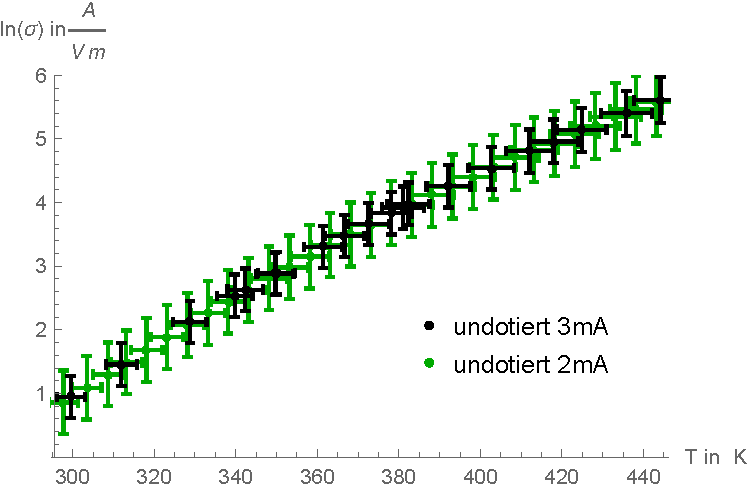
\includegraphics[width=0.9\linewidth]{IMAGE/M2_Stromvergleich.pdf}
	\caption{Vergleich des undotierten Germaniums bei Änderung des Probestromes $I_{Probe}$}
	\label{fig:M2_4}
\end{figure} 

In Abbildung \ref{fig:M2_4} ist zusehen, dass der Probestrom keinen Einfluss auf die Steigung hat. Dies ist anschaulich klar, denn die Steigung ist die Energielücke $E_{G}$, die vom Probestrom unabhängig sein sollte. Dies wird im folgenden Quantitativ durch Ermittelung dieser Konstante gezeigt.\\

\begin{figure}[H]
	\centering
	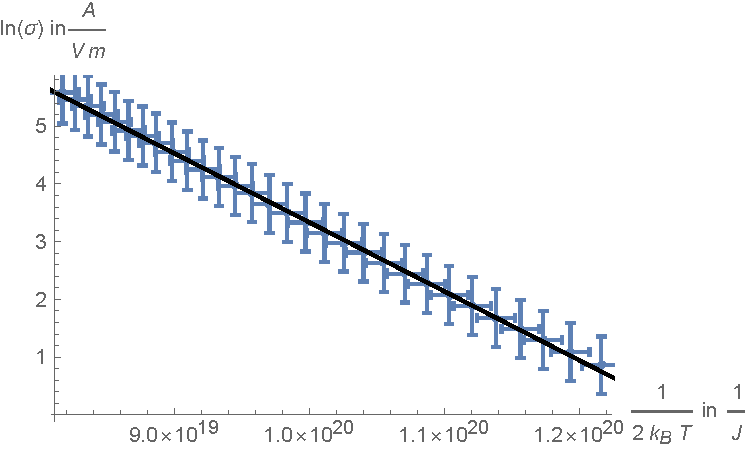
\includegraphics[width=0.9\linewidth]{IMAGE/M1_2mA.pdf}
	\caption{Linearer Fit mit Gewichtung $\frac{1}{(a*x_{error})^2+(y_{error})^2}$ für $I_{Probe}=2mA$:\\ $f(x)=(-1.1948 \pm 0.0065)\times 10^{-19}x + Ln((4.33 \pm 0.28)\times 10^{6})$}
	\label{fig:M1_1}
\end{figure} 

Für den Fit wurde eine Näherung der Steigung$a=1.1944\times 10^{-19}$ verwendet.\\
Der Porportionalitätsfaktor wurde als $E_{G}=(-1.1948 \pm 0.0065)\times 10^{-19} [J]$ mit einer Genauigkeit von 0.55\% bestimmt und $\sigma_{0}=(4.33 \pm 0.28)\times 10^{6}$ mit einer Genauigkeit von 6.4\%.\\

\begin{figure}[H]
	\centering
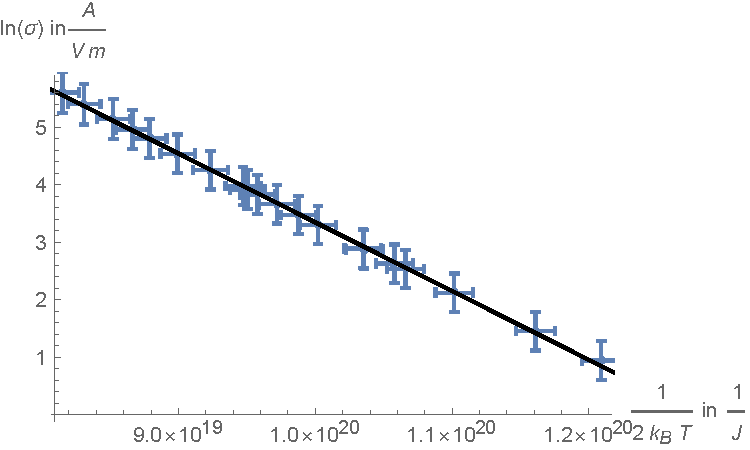
\includegraphics[width=0.9\linewidth]{IMAGE/M1_3mA.pdf}
	\caption{Linearer Fit mit Gewichtung für $I_{Probe}=3mA$:\\ $f(x)=(-1.1961 \pm 0.0076)\times 10^{-19}x + Ln((4.45 \pm 0.33)\times 10^{6})$}
	\label{fig:M1_2}
\end{figure} 

Für den Fit wurde als Gewichtung $\frac{1}{(a*x_{error})^2+(y_{error})^2}$ eine Näherung der Steigung  $a=1.1953\times 10^{-19}$ verwendet.\\
Der Porportionalitätsfaktor wurde als $E_{G}=(-1.1961 \pm 0.0076)\times 10^{-19} [J]$ mit einer Genauigkeit von 0.63\% bestimmt und $\sigma_{0}=(4.45 \pm 0.33)\times 10^{6}$ mit einer Genauigkeit von 7.4\%.\\

\subsubsection{Vergleich}

Bei $I_{Probe}=2mA$: $E_{G}=(-1.1948 \pm 0.0065)\times 10^{-19} [J]$ und $\sigma_{0}=(4.33 \pm 0.28)\times 10^{6}$.\\
Bei $I_{Probe}=3mA$: $E_{G}=(-1.1961 \pm 0.0076)\times 10^{-19} [J]$ und $\sigma_{0}=(4.45 \pm 0.33)\times 10^{6}$.\\
Diese sind miteinander verträglich, sodass eine Abhängigkeit der Energielücke vom Probestrom in diesen Größenordnungen nicht nachweisbar ist.

\subsection{M2}

\subsubsection{Messwerte}
\begin{table}[H]
\centering
\begin{tabular}{|c||c|c|c|c|c|c|c|c|c|}
\hline
T [K] & 299.25 & 303.15 & 308.15 & 313.15 & 318.15 & 323.45 & 328.15 & 333.15 & 338.15 \\
 U [V] & 0.764 & 0.759 & 0.797 & 0.806 & 0.832 & 0.85 & 0.828 & 0.791 & 0.835 \\
 \hline
 T [K] & 343.15 & 348.15 & 353.15 & 358.15 & 363.15 & 368.15 & 373.45 & 378.15 & 383.15 \\
 U [V] & 0.796 & 0.864 & 0.781 & 0.732 & 0.706 & 0.69 & 0.666 & 0.551 & 0.512 \\
 \hline
 T [K] & 388.45 & 393.15 & 398.15 & 403.15 & 408.15 & 413.15 & 418.15 & 423.65 & 428.15 \\
 U [V] & 0.472 & 0.486 & 0.437 & 0.39 & 0.349 & 0.312 & 0.279 & 0.245 & 0.223 \\
 \hline
 T [K]& 433.15 & 438.75 & 443.15 & & & & & & \\
U [V] & 0.199 & 0.176 & 0.160 & & & & & & \\
 \hline
\end{tabular}
\caption{n-dotiertes Germanium: Spannung in Abhängigkeit von der Temperatur bei $I_{Probe}=20mA$}
\end{table}  

\begin{table}[H]
\centering
\begin{tabular}{|c||c|c|c|c|c|c|c|c|c|}
\hline
T [K] & 298.95 & 314.55 & 324.45 & 332.35 & 353.35 & 365.55 & 374.95 & 383.45 & 391.35 \\
 U [V] & 0.88 & 0.98 & 1.04 & 1.04 & 1.018 & 0.929 & 0.704 & 0.698 & 0.632 \\
 \hline
 T [K]& 402.45
   & 406.05 & 421.65 & 436.25 & & & & & \\
U [V] & 0.469 & 0.36 & 0.282
   & 0.195 & & & & & \\
 \hline
\end{tabular}
\caption{p-dotiertes Germanium: Spannung in Abhängigkeit von der Temperatur bei $I_{Probe}=20mA$}
\end{table} 

\subsubsection{Fehlergrenzen}
Aus diesen Werten werden mittels $\sigma=\frac{I}{U}\frac{c}{b *d}$ die Leitfähigkeit berechnet, wobei $c=20 \times 10^{-3}$, $b=10 \times 10^{-3}$ und $d=1 \times 10^{-3}$. Die Fehlergrenzen der Spannung werden vom Hersteller mit (.5\% + 3dgts) angegeben, in diesem Fall, da die Auflösung 0.001V ist (.5\% + 0.003V). Fehlergrenzen der gemessenen Temperatur(in \celsius) sind (2\% + 3°C). Die Fehlergrenze des Stromes liegt bei 1mA. Weiterhin werden mittels Fehlerfortpflanzung die Fehler von Größen, die mit diesen Größen errechnet werden, bestimmt.\\

\subsubsection{Auswertung}
\begin{figure}[H]
	\centering
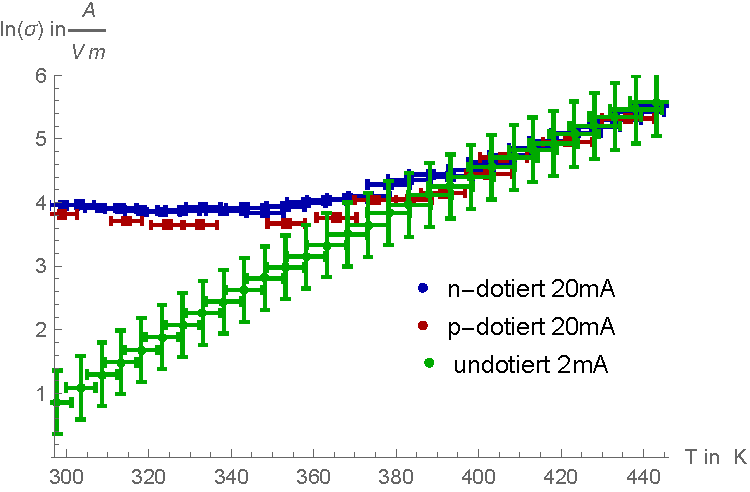
\includegraphics[width=0.9\linewidth]{IMAGE/M2_all.pdf}
	\caption{Vergleich der Leitfähigkeit in Abhängigkeit zur Temperatur von\\ n-,p- und undotiertem Germanium}
	\label{fig:M2_1}
\end{figure} 

Die aufgenommenen Messkurve zeigt dieselbe Abhängigkeit der Leitfähigkeit des un- und n-dotierten Germaniums von der Temperatur wie die Abbildung im Praktikumsbericht. Dort wurde die Skala logarithmiert, hier die Werte der Leitfähigkeit. Zusätzlich wurde im Versuch die Messkurve zum p-dotierten Germanium aufgenommen.\\
Die Leitfähigkeit ist von der Besetzung des Leitungsbandes abhängig. Diese wiederum hängt von der Energielücke zwischen Valenz- und Leitungsband der Probe und von der thermischen Energie (Temperatur) der Probe ab. Je höher die thermische Energie, desto wahrscheinlicher ist es für Elektronen die Energielücke zu überwinden und in das Leitungsband zu gelangen.\\
Die dotierten Proben haben schon bei Zimmertemperatur eine hohe Leitfähigkeit, denn die thermische Energie reicht aus um viele Elektronen ins Leitungsband zu bringen.\\ 
Bei dem undotierten Material hängt die Leitfähigkeit von der Besetzungswahrscheinlichkeit für endliche Temperaturen (diese ist exponentiell) ab. Bei den dotierten Material ist die Löcherkonzentration und Elektronenkonzentration im Bereich der Zimmertemperatur nicht gleich, das Modell also in diesem Bereich nicht anwendbar, erst bei höheren Temperaturen ist der Unterschied der Konzentrationen nicht mehr ausschlaggebend. \\

\begin{figure}[H]
	\centering
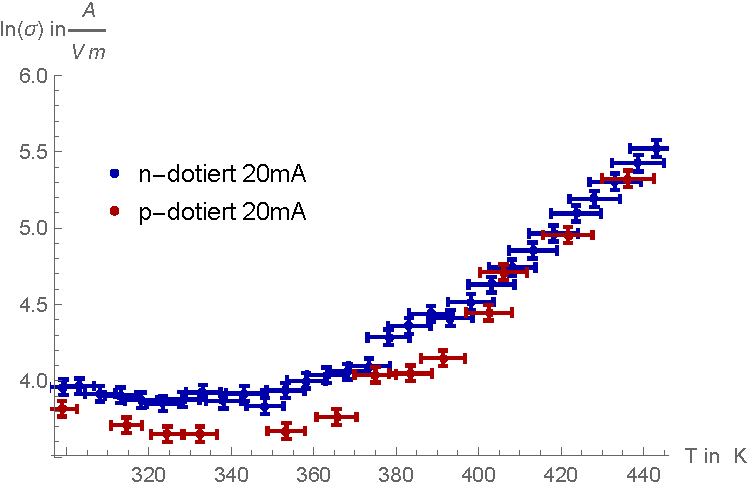
\includegraphics[width=0.9\linewidth]{IMAGE/M2_npVergleich.pdf}
	\caption{Vergleich der Leitfähigkeit in Abhängigkeit zur Temperatur von\\ n- und p-dotiertem Germanium}
	\label{fig:M2_3}
\end{figure} 

Es ist zweckmäßig die dotierten Proben in getrenntem Diagramm zu betrachten, um Unterschiede herauszustellen.\\
Das p-dotierte Germanium hat bei ungefähr 340K sein Minimum an Leitfähigkeit und ist im Allgemeinen weniger leitfähig als das n-dotierte. \\

\subsection{M3.1}
\subsubsection{Messwerte}
\begin{table}[H]
\centering
\begin{tabular}{|c||c|c|c|c|c|c|c|c|}
\hline
$I_{Probe}$ [A] & 0. & 0.003 & 0.0054 & 0.01 & 0.0151 & 0.02 & 0.0252 & 0.0298 \\
 U [V] & 0. & 0.002 & 0.0036 & 0.0066 & 0.01 & 0.0132 & 0.0166 & 0.0197 \\
 \hline
\end{tabular}
\caption{n-dotiertes Germanium: Hallspannung in Abhängigkeit vom Probestrom bei $I_{Spule}= 1.97$}
\end{table} 

\begin{table}[H]
\centering
\begin{tabular}{|c||c|c|c|c|c|c|c|c|}
\hline
$I_{Probe}$ [A] & 0. & 0.003 & 0.0051 & 0.0099 & 0.015 & 0.0203 & 0.0252 & 0.0297 \\
 U [V] & 0. & 0.0021 & 0.0036 & 0.007 & 0.0106 & 0.0144 & 0.0179 & 0.0211 \\ 
 \hline
\end{tabular}
\caption{p-dotiertes Germanium: Hallspannung in Abhängigkeit vom Probestrom bei $I_{Spule}= 1.97$}
\end{table} 

\subsubsection{Fehlergrenzen}
Die Fehlergrenzen der Spannung $U_{H}$ werden vom Hersteller mit (.5\% + 3dgts) angegeben, in diesem Fall, da die Auflösung 0.001V ist (.5\% + 0.003V). Fehlergrenzen der gemessenen Temperatur(in °C) sind (2\% + 3°C). Die Fehlergrenze des Stromes $I_{Probe}$ liegt bei 1mA.\\

\subsubsection{Auswertung}
\begin{figure}[H]
	\centering
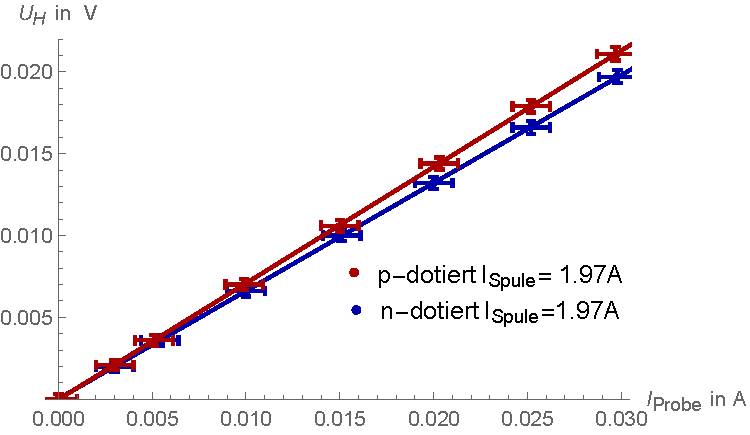
\includegraphics[width=0.9\linewidth]{IMAGE/M31_Fit.pdf}
	\caption{Linearer Fit mit Gewichtung $\frac{1}{(a_{i}*x_{error})^2+(y_{error})^2}$ p-dotiert bei $T=300.0K$ und n-dotiert bei $T=299.0K$:\\ $f_{p}(x)=(0.71085 \pm 0.00073)x + (-0.000027 \pm 0.000012)$\\ $f_{n}(x)=(0.65962 \pm 0.00087)x + (-0.000016 \pm 0.000014)$}
	\label{fig:M3_1_1}
\end{figure} 


Für den Fit  des p-Dotierten wurde eine Näherung der Steigung  $a_{p}=0.71065$  und für den Fit des n-Dotierten verwendet $a_{n}=0.65964$.\\
\\
Bei $T=300.0K$ wurde für das p-dotierte Germanium  $R_{H}\frac{B}{d}=(0.71085 \pm 0.00073) [\frac{V}{A}]$ mit einer Genauigkeit von 0.1\% bestimmt und\\
der Systematische Fehler $(-0.000027 \pm 0.000012)$ mit einer Genauigkeit von 45\%.\\
\\
Bei $T=299.0K$ wurde für das n-dotierte Germanium $R_{H}\frac{B}{d}=(0.65962 \pm 0.00087) [\frac{V}{A}]$ mit einer Genauigkeit von 0.1\% bestimmt und\\ der Systematische Fehler $(-0.000016 \pm 0.000014)$ mit einer Genauigkeit von 87.5\%.\\


\listoffigures
\listoftables

\begin{thebibliography}{99}
	\bibitem{Schaltung1} \textsc{Saure aus Wikimedia Commons}, \emph{Gleichrichter-Schaltung mit Glättung} (26. August 2009) (Stand: 08.03.2018) \url{https://commons.wikimedia.org/w/index.php?title=File:Gleichrichter-Schaltung.svg&oldid=291347227&uselang=de}
\end{thebibliography}

\end{document}
